\clearpage
\section{Motorcontroller}

The chassis used for the rover has 4 pre-installed DC motors, which are all four used for movement. To control the direction of the rover a Pololu DRV8833 motor controller has been connected to the motors and the Raspberry Pi. The motor controller is in charge of operating the steering-, forward- and reversing motion of the rover.

\begin{figure}[H]
	\centering
	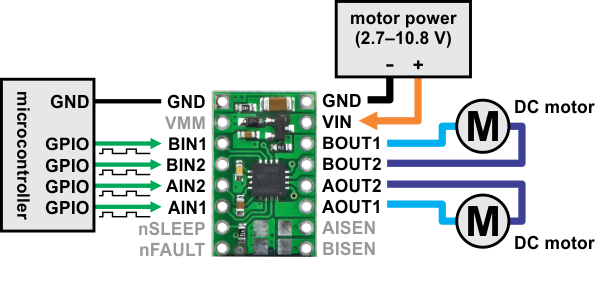
\includegraphics[width=.8\linewidth]{images/DRV8833.png}
	\caption{Pololu DRV8833\cite{DRV8833pic}}
	\label{fig:polulu}
\end{figure}

The driver uses a 2.7-10.8V supply voltage to operate, which is supplied to the motor controller by an external battery pack. This battery-pack is used to power the motor controller and the four DC motors on the rover. The DRV8833 has two separate DC motor outputs labeled as \textit{BOUT} and \textit{AOUT}, that can be independently controlled by their matching inputs from the microcontroller, since this rover uses 4 DC motors, each of the outputs from the motor controller will be connected to 2 DC motors.

The advantage of this particular motor controller is the fact that it supports analog and digital inputs. Since the Raspberry Pi has no analog outputs the controller will be given digital inputs. 

\begin{table}[H]
	\centering
	\begin{tabular}{|c|c|c|c|}
		\hline
		xIN1 & xIN2 & xOUT1 & xOUT2 \\ \hline
		0    & 0    & Z     & Z     \\ \hline
		0    & 1    & H     & L     \\ \hline
		1    & 0    & L     & H     \\ \hline
		1    & 1    & L     & L     \\ \hline
	\end{tabular}
	\caption{The truth table for the outputs}
	\label{motorcontrollertruthtabel}
\end{table}

Table \ref{motorcontrollertruthtabel} shows the possible combinations of pins to achieve different desired directions/states, where the pins must be set to high and low according to what is the direction of choice. To turn the rover, the A and B inputs will be flipped, so that when \textit{AOUT} goes forward, the \textit{BOUT} reverses, which results in the rover turning in its place.
The input pins on the motor controller also allow for control with PWM (Pulse Width Modulation), which will change the length of the duty cycle and influence the speed of which the rover is moving at\cite{DRV8833}.

\begin{figure}[H]
	\centering
	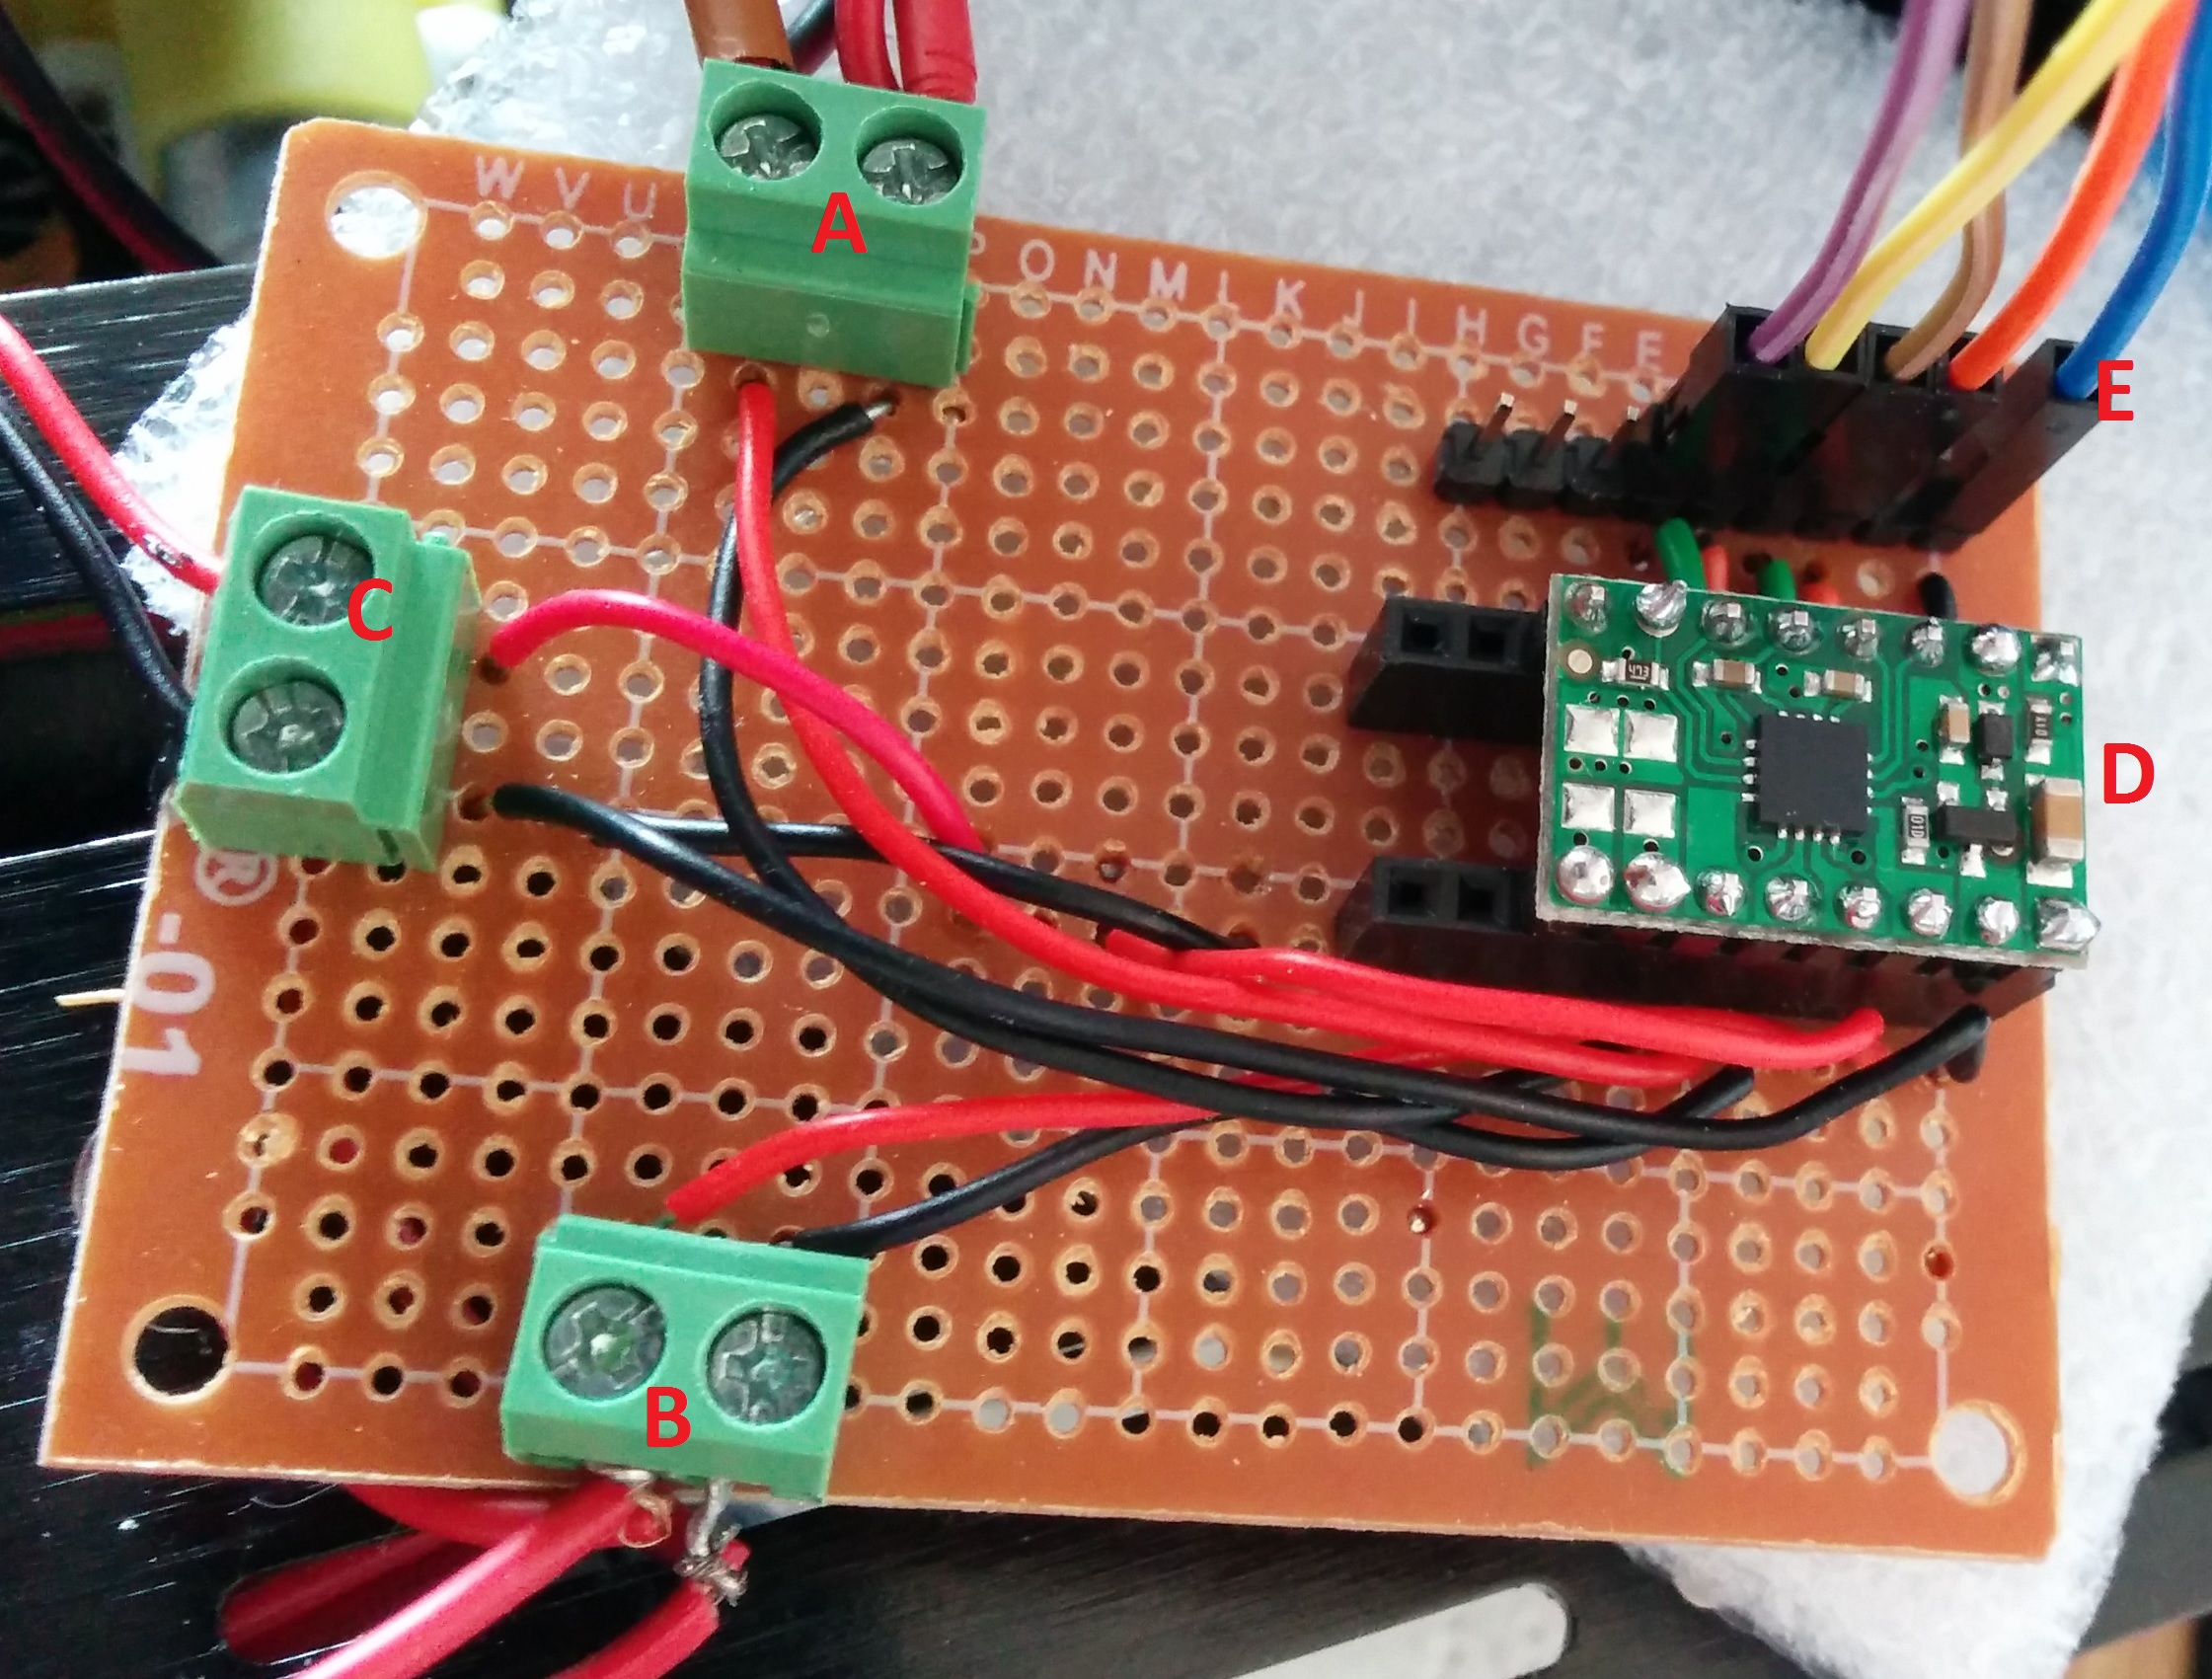
\includegraphics[width=.5\linewidth]{images/labelled.jpg}
	\caption{Custom board for the motor controller}
	\label{fig:customboardmc}	
\end{figure}

To enable easier access to the pins on the motor controller, a custom board has been created for ease of use. The green terminals, A and B, are connection terminals for the \textit{AOUT} and \textit{BOUT} respectively. The terminal C is for the battery pack that supplies the voltage to the motor controller and the DC motors, which in this case is 5 AA batteries. The label D is the Pololu DRV8833 and the final label E are the connections to the Raspberry Pi. 

Operating the motor controller requires 5 pins from the Raspberry Pi, 4 to control the input pins on the DRV8833 and a ground pin. Since we are controlling the motor controller using HIGH and LOW, the controller can be connected to any of the regular digital GPIO pins.